\section{Overview}
Using the different concepts introduced in the previous chapters we built a pipeline from CAD design via topology optimization back to CAD. An overview over the implementation workflow is shown in \autoref{fig:pipeline}. It describes the different steps and the transformations applied on the geometry at whose implementation details we will now look more closely.
\begin{figure}[ht]
\begin{center}
		\begin{tikzpicture}[remember picture, auto,
    block/.style={
      rectangle,
      draw=blue,
      thick,
      fill=blue!20,
      text width=5em,
      align=center,
      rounded corners,
      minimum height=2em
    },
    block1/.style={
      rectangle,
      draw=blue,
      thick,
      fill=blue!20,
      text width=5em,
      align=center,
      rounded corners,
      minimum height=2em
    },
    line/.style={
      draw,thick,
      -latex',
      shorten >=2pt
    },
    cloud/.style={
      draw=red,
      thick,
      ellipse,
      fill=red!20,
      minimum height=1em
    }]
        \node [anchor=north,inner sep=0pt] [xshift=-4cm,yshift=0.7cm,inner sep=0pt](N1)
                {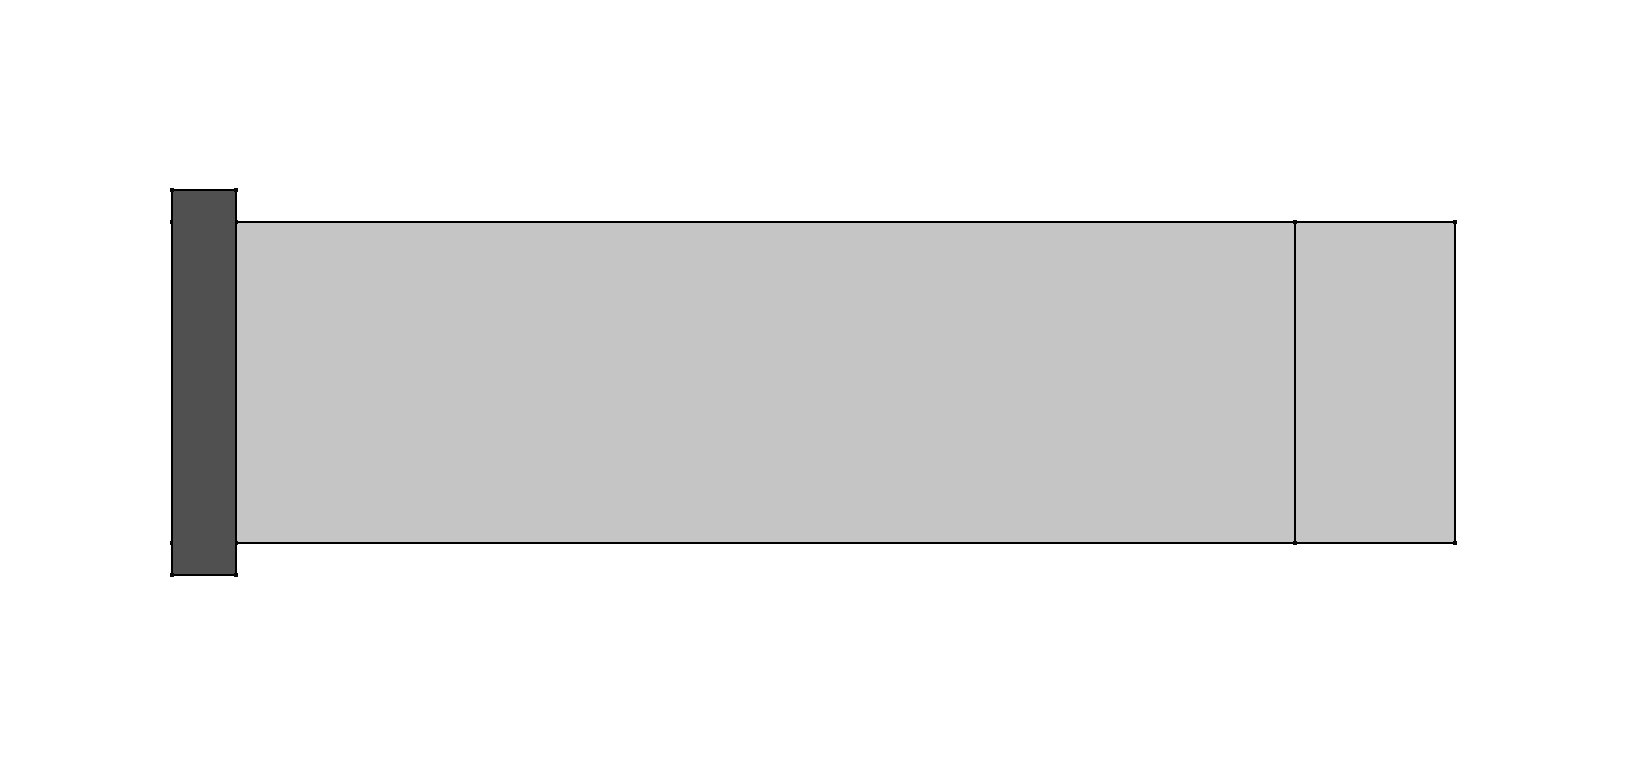
\includegraphics[scale=0.1]{Pictures/CADO_Overview/Back2CAD1.png}};
        \node [below =of N1,inner sep=0pt] [xshift=0cm,yshift=1cm,inner sep=0pt](N5)
				{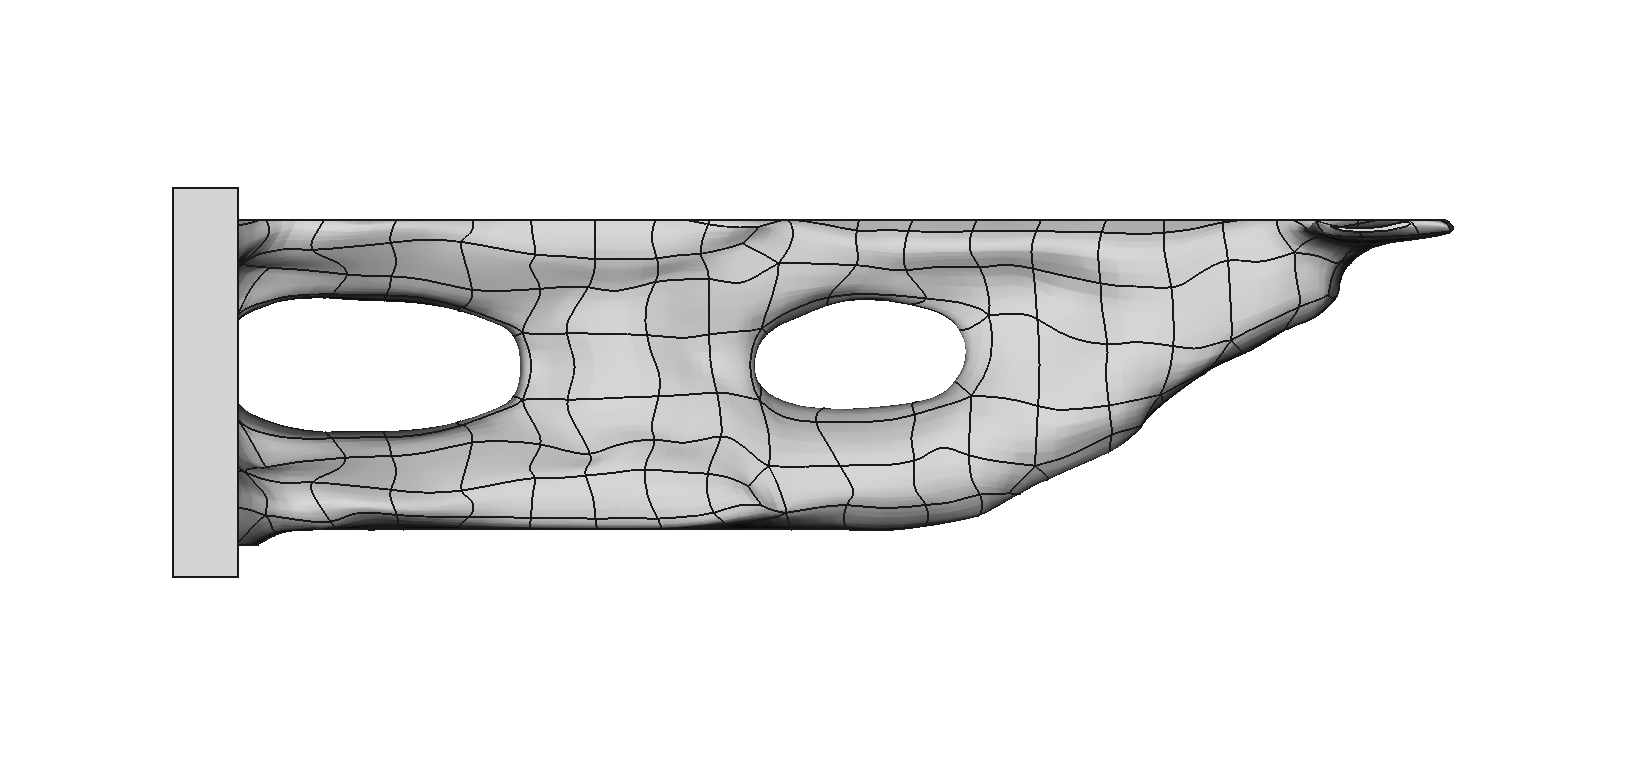
\includegraphics[scale=0.1]{Pictures/CADO_Overview/Back2CAD6.png}};
      	%\path[thick, ->,] (N5) edge [bend left] (N1); %node[yshift=-1.8cm, xshift = -0.1cm]{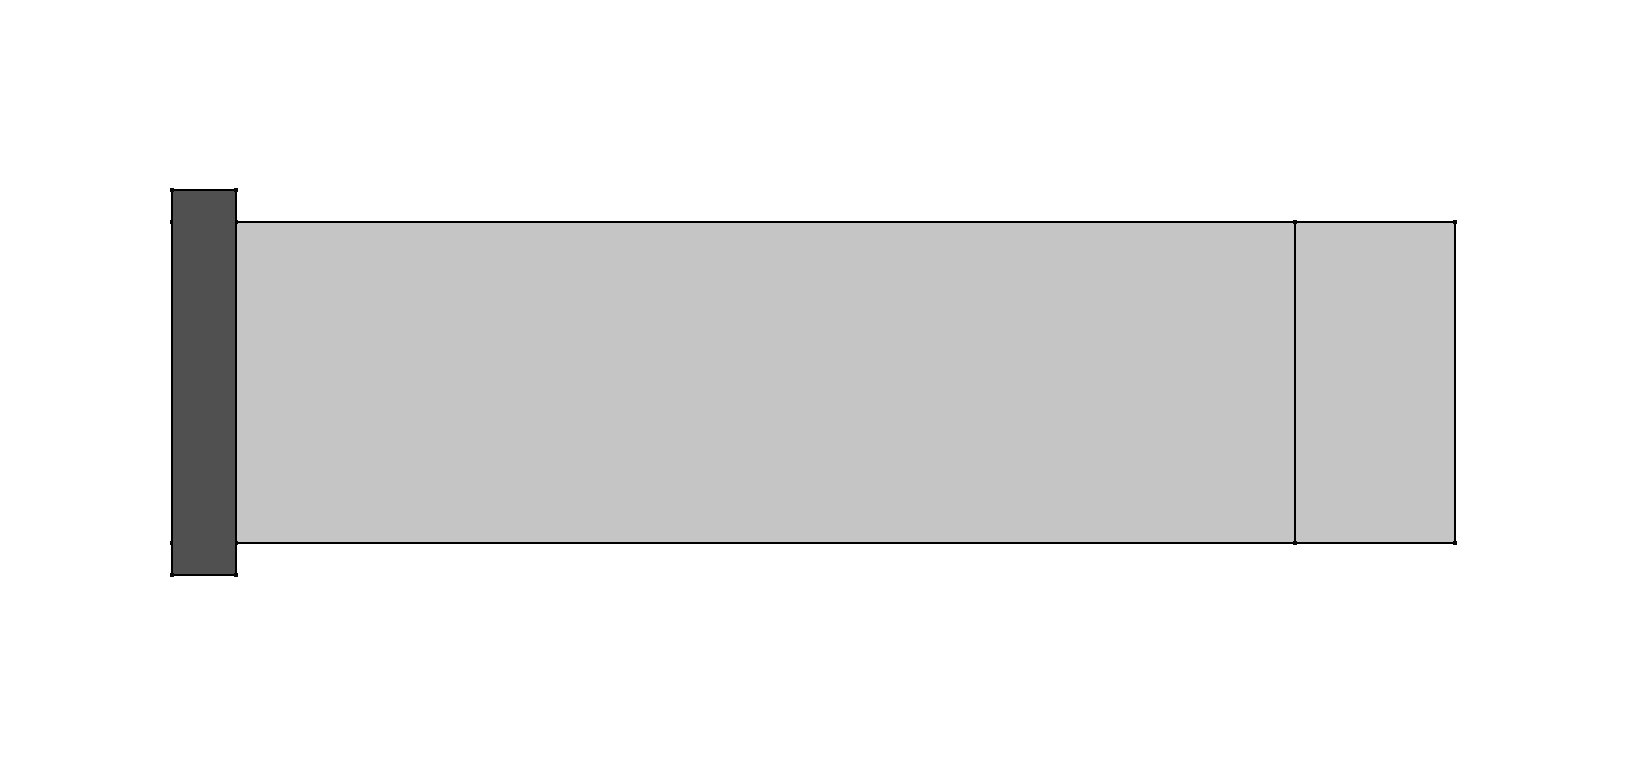
\includegraphics[scale=0.1]{Pictures/CADO_Overview/Back2CAD1.png}};
        \node [right =of N1,inner sep=0pt] [xshift=-2.5cm,yshift=2cm, inner sep=0pt](N2)             
                {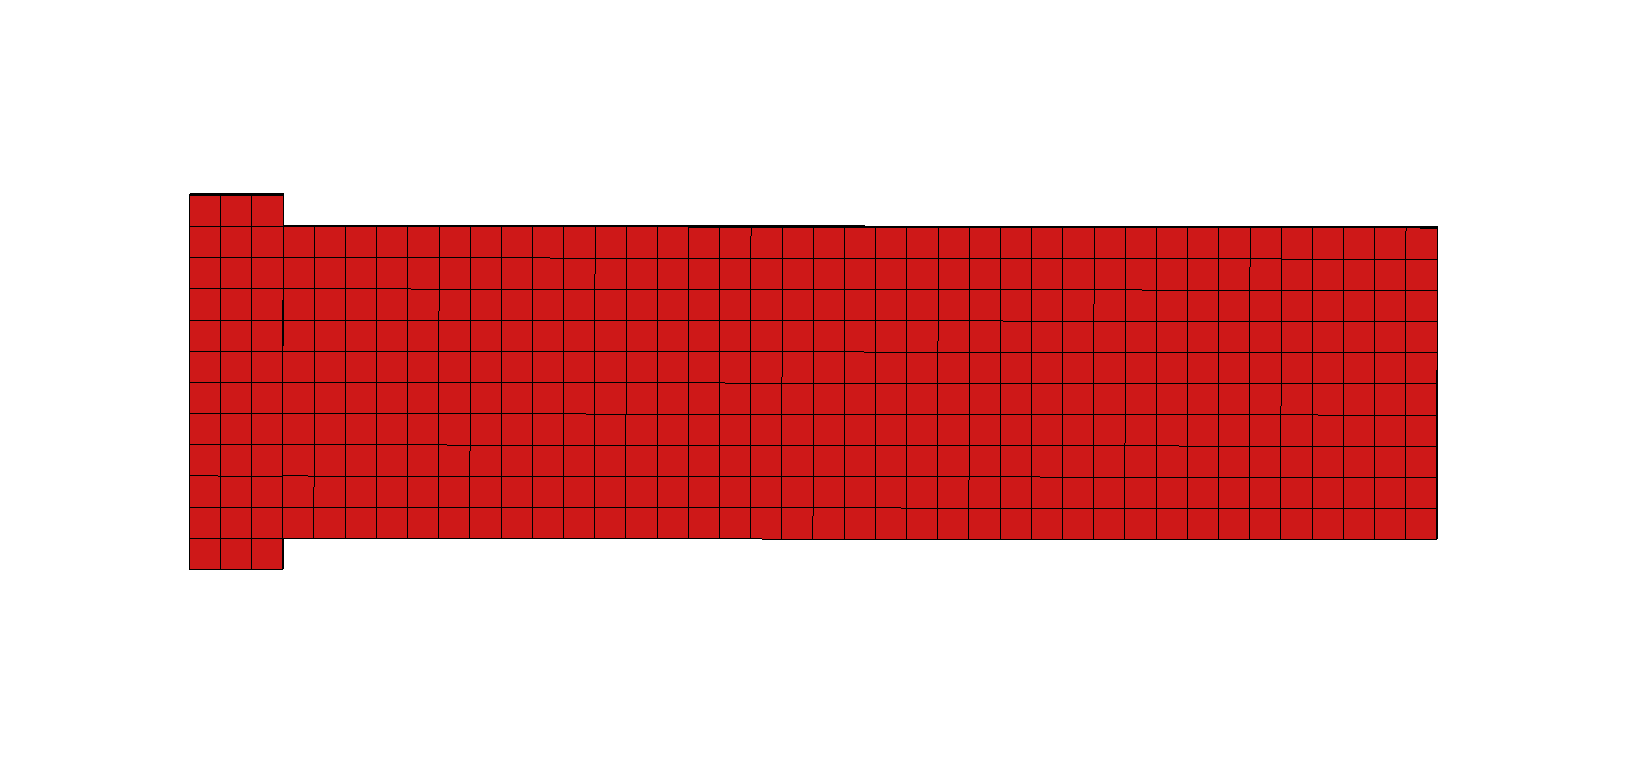
\includegraphics[scale=0.1]{Pictures/CADO_Overview/Back2CAD2.png}};
        \path[thick, ->] (N1) edge [bend left] (N2) node[yshift=0cm, xshift = -2.7cm]{(a)};
        \node [right =of N2,inner sep=0pt] [xshift=-2cm,yshift=-2cm, inner sep=0pt](N3) 
                {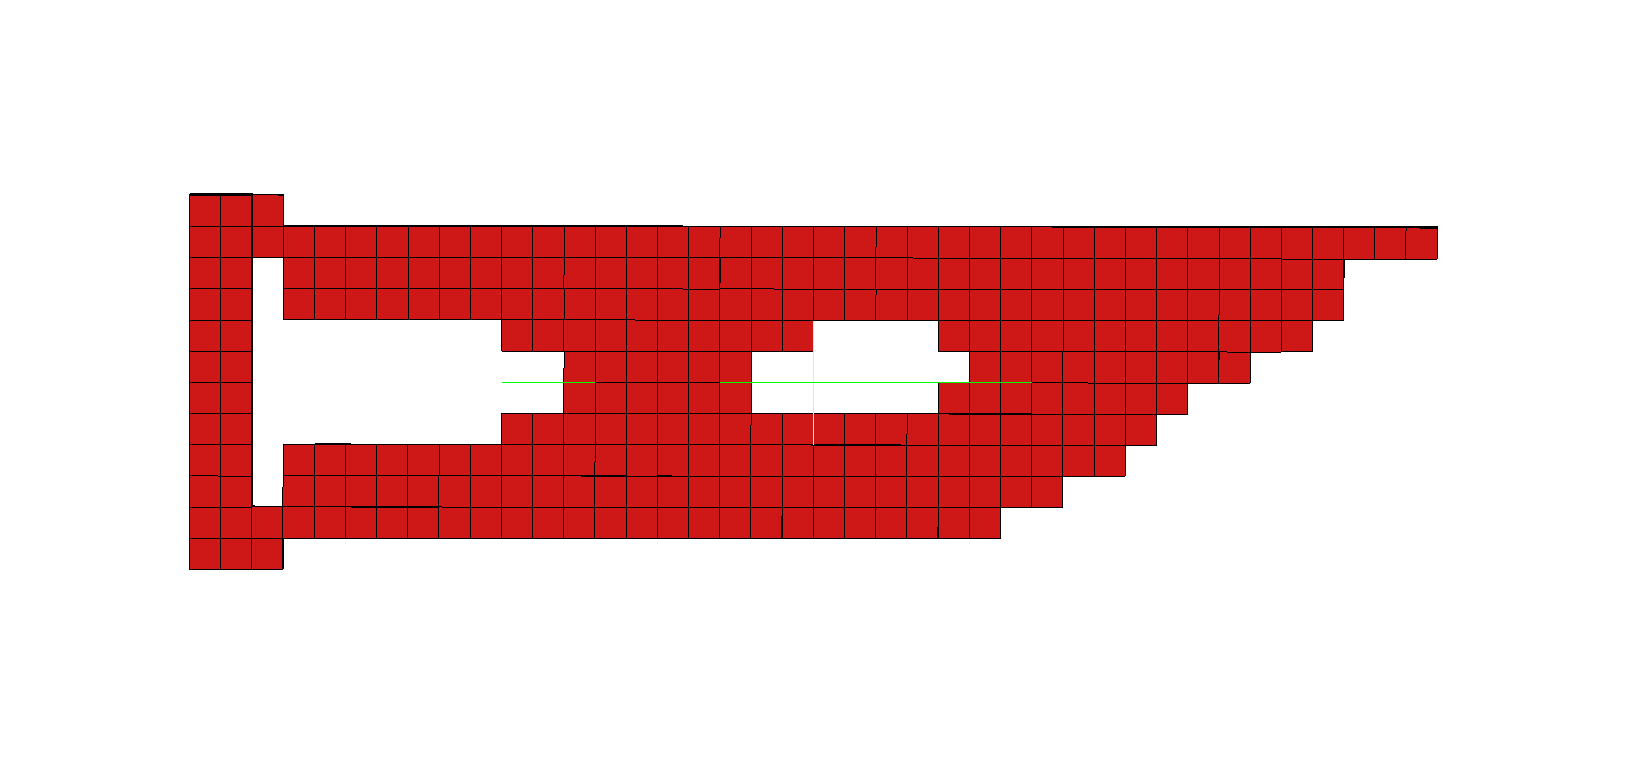
\includegraphics[scale=0.1]{Pictures/CADO_Overview/Back2CAD3.png}};
        \path[thick, ->] (N2) edge [bend left] (N3) node[yshift=1cm, xshift = 0.1cm]{(b)};
        \node [below =of N3,inner sep=0pt] [xshift=-0cm,yshift=1cm, inner sep=0pt](N4)
                {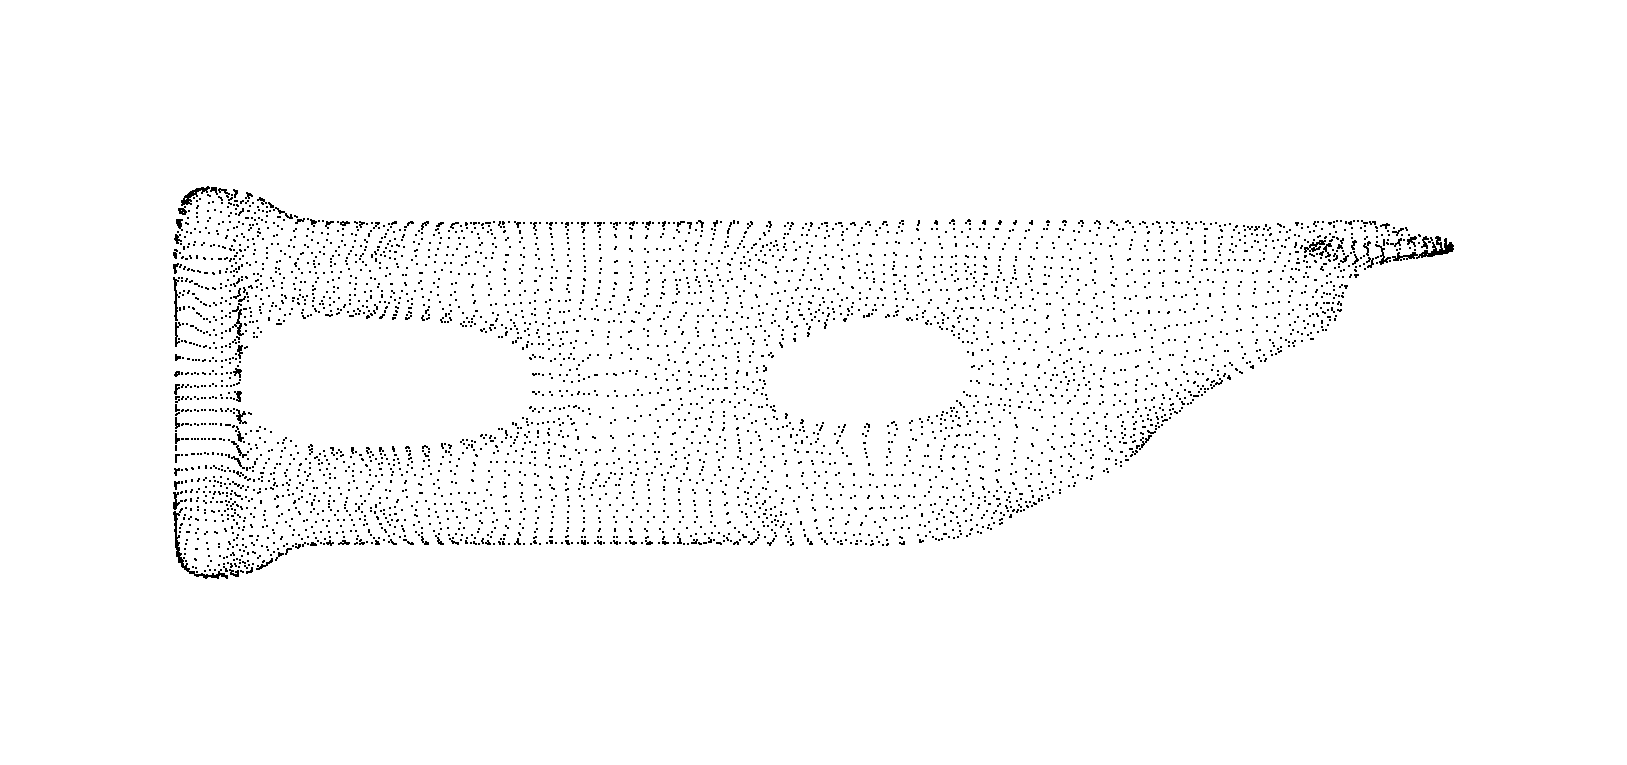
\includegraphics[scale=0.1]{Pictures/CADO_Overview/Back2CAD4.png}};
        \coordinate (N31) at (-0.9,-1);
        \coordinate (N32) at ($(N3)+(N31)$);
        \coordinate (N41) at (-0.9,1);
        \coordinate (N42) at ($(N4)+(N41)$);
        \draw[thick, ->] (N32) -- (N42) node[yshift=1.8cm, xshift = 3.5cm]{(c)};
        \node [right =of N5,inner sep=0pt] [xshift=-2.2cm,yshift=-2cm, inner sep=0pt](N6)
                {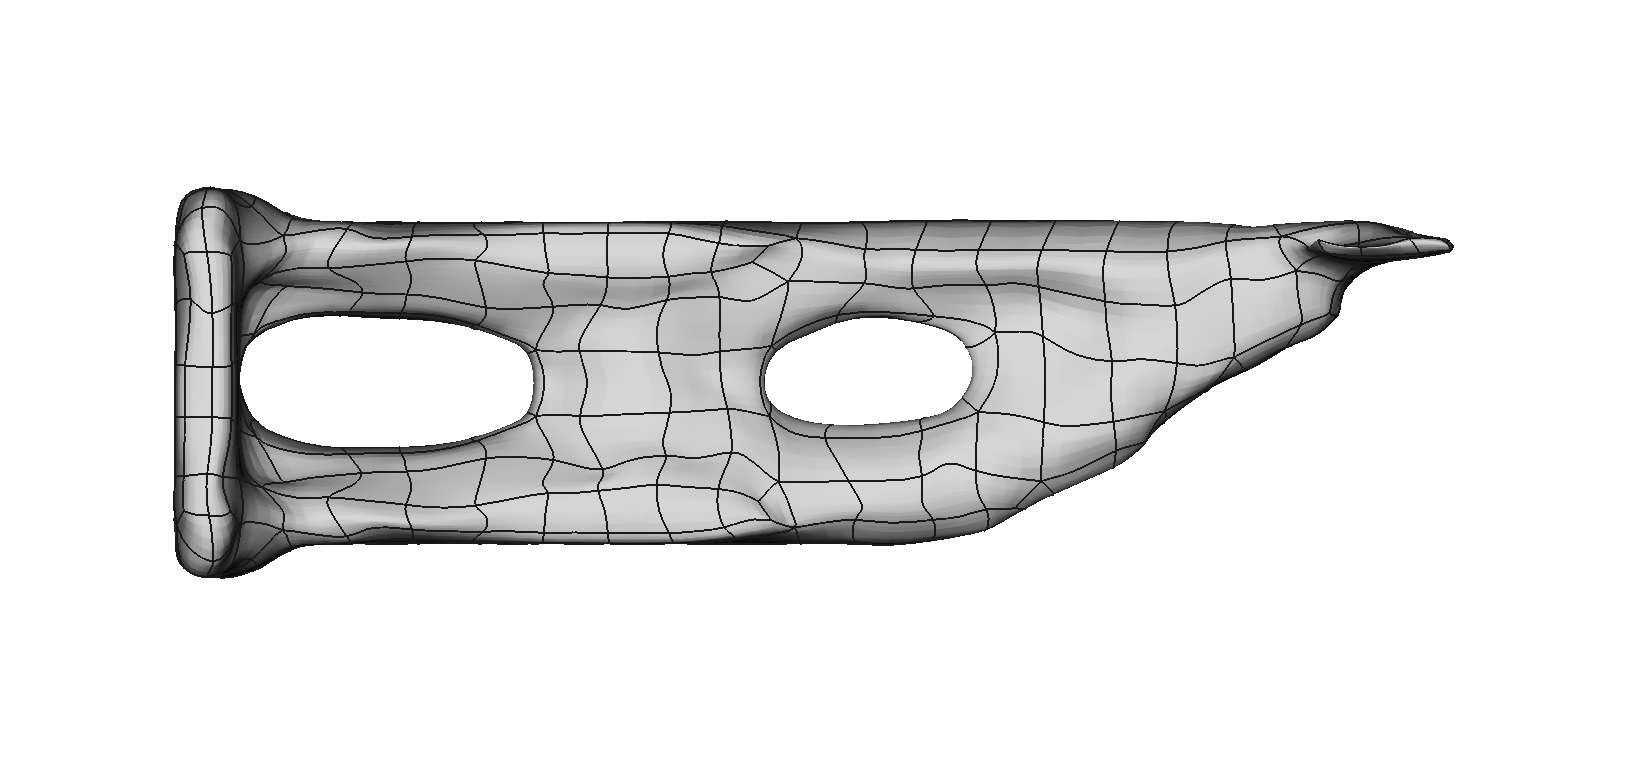
\includegraphics[scale=0.1]{Pictures/CADO_Overview/Back2CAD5.png}};
        \path[thick, ->] (N4) edge [bend left] (N6) node[yshift=0.1cm, xshift = 2.6cm]{(d)};
        \path[thick, ->] (N6) edge [bend left] (N5) node[yshift=-1cm, xshift = -0.1cm]{(e)} node[yshift=2cm, xshift = -7.22cm]{(f)};
        \end{tikzpicture}
        \caption{Starting off with an input geometry (a), the first step is voxelization, in which we convert the CAD geometry into a three-dimensional voxel grid (b). This grid then undergoes topology optimization (c) from which the points for surface fitting are computed (d). This is followed by construction of NURBS surfaces through these points (e). Finally, post-processing with fixtures and optimization domain limits results in the final geometry (f).}
        \label{fig:pipeline}
	\end{center}
\end{figure}
